\documentclass{beamer}
\usetheme{Madrid}
\usecolortheme{beaver}
\setbeamertemplate{navigation symbols}{}
\setbeamertemplate{footline}[frame number]

\usepackage[utf8]{inputenc}
\usepackage[T1]{fontenc}
\usepackage{amsmath,amssymb}
\usepackage{graphicx}
\usepackage{booktabs}
\usepackage{xcolor}
\usepackage{listings}
\usepackage{tikz} % Added for diagrams
\usetikzlibrary{arrows.meta, positioning, shapes.geometric} % Added for diagrams

% Title metadata
\title{Mixed FEM–PINN Domain Decomposition Solver}
\subtitle{Neumann–Dirichlet Schwarz Iteration for 1D Heat Conduction}
\author{Yehua HE}
\institute{University of Strasbourg}
\date{May 2025}

\begin{document}

% Slide 1
\begin{frame}[plain]
  \titlepage
\end{frame}

% Slide 2
\begin{frame}{Outline}
  \tableofcontents % This will automatically update if sections/slides change before it
\end{frame}

% Slide 3
\section{Motivation}
\begin{frame}{Motivation: Why Hybrid FEM–PINN?}
\begin{figure}
    \centering
    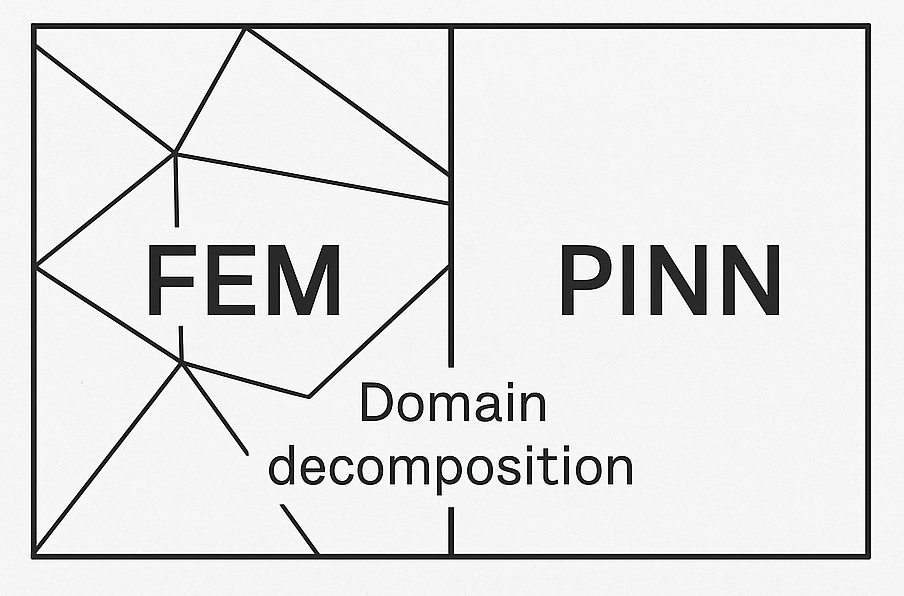
\includegraphics[width=0.45\linewidth]{assets/slide-image-1.png} 
\end{figure}  
  \begin{itemize}
    \item \textbf{FEM:} Accurate, stable, mesh-based, but requires full model knowledge. 
    \item \textbf{PINN:} Flexible, mesh-free, handles partial/noisy data, can learn physics. 
    \item \textbf{Limitations to Address:}
    \begin{itemize}
      \item FEM: Challenges with unknown or highly complex physics.
      \item PINN: Can face slow convergence or instability for stiff problems.
    \end{itemize} 
    \item \textbf{Our Solution:} Combine strengths via domain decomposition. 
    \item \textbf{Coupling Tool:} Schwarz-type Neumann–Dirichlet iteration.
  \end{itemize}
\end{frame}

% Slide 4
\section{Mathematical Model}
\begin{frame}{Mathematical Model \& Domain Split}
  \[
    \partial_t u - \alpha\,\partial_{xx}u = 0,
    \quad x\in[0,1],\;t\in[0,T].
  \]
  \begin{itemize}
    \item Initial: \(u(x,0)=\sin(\pi x)\), Boundary: \(u(0,t)=u(1,t)=0\). 
    \item Exact solution (for validation): \(u_{\rm exact}=e^{-\alpha\pi^2t}\sin(\pi x)\). 
    \item Split at interface \(x_m=0.4\):
      \begin{itemize}
        \item FEM on \([0,x_m]\) (Left subdomain)
        \item PINN on \([x_m,1]\) (Right subdomain)
      \end{itemize}
  \end{itemize}
\begin{figure}
    \centering
    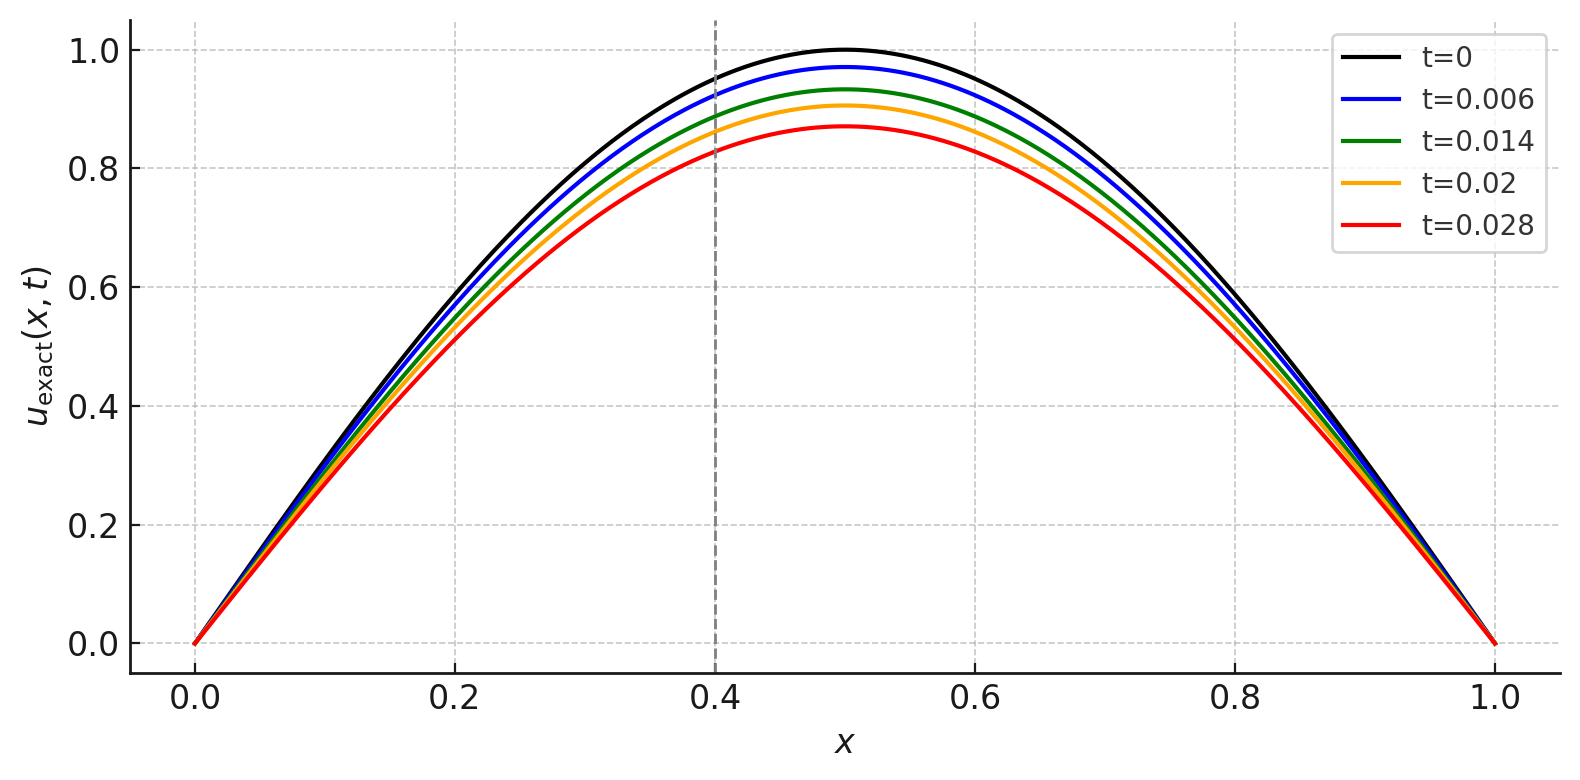
\includegraphics[width=0.7\linewidth]{assets/slide-image-2.png} 
\end{figure}
\end{frame}

% Slide 5
\begin{frame}{Interface Coupling Conditions}
  At the interface \(x=x_m\), we enforce continuity:
  \begin{itemize}
    \item \textbf{FEM (receives Neumann BC from PINN)}: 
      The flux from PINN is applied to FEM:
      \[ -\alpha\,\partial_x u\big|_{x_m^-}^{\text{FEM}} = q_I(t) \quad (\text{from PINN}) \] 
    \item \textbf{PINN (receives Dirichlet BC from FEM)}: 
      The temperature from FEM is applied to PINN:
      \[ u(x_m,t)^{\text{PINN}} = u_I(t) \quad (\text{from FEM}) \]
  \end{itemize}
  \vspace{0.5em}
  \begin{center}
  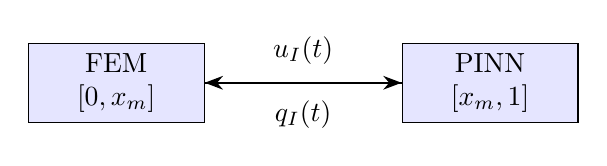
\begin{tikzpicture}[node distance=2.5cm, auto,
    solverbox/.style={rectangle, draw, fill=blue!10, minimum height=1cm, minimum width=2.2cm, text centered, text width=2cm}, 
    dataflow/.style={-Stealth, thick}] 
    \node[solverbox] (fem) {FEM \\ $[0, x_m]$};
    \node[solverbox, right=of fem] (pinn) {PINN \\ $[x_m, 1]$};
    \draw[dataflow] (fem.east) -- (pinn.west) node[midway, above, sloped, yshift=1mm] {\(u_I(t)\)};
    \draw[dataflow] (pinn.west) -- (fem.east) node[midway, below, sloped, yshift=-1mm] {\(q_I(t)\)};
  \end{tikzpicture}
  \end{center}
  
  \textit{Alternate updates of \(u_I(t)\) and \(q_I(t)\) drive the system to a consistent global solution.}
\end{frame}

% Slide 6
\section{Schwarz Iteration}
\begin{frame}{Neumann–Dirichlet Schwarz Iteration}
  \begin{enumerate}
    \item \textbf{Initialization:} Choose initial guess for interface flux \(q_I^{(0)}(t)\). 
    \item \textbf{Iteration Loop} (for \(k=0,1,\dots\)):
      \begin{itemize}
        \item[(a)] \textbf{FEM Solve:} Given \(q_I^{(k)}(t)\), solve FEM on \([0,x_m]\) to obtain \(u_I^{(k)}(t)\). 
        \[ \text{FEM}(q_I^{(k)}) \quad \xrightarrow{\text{solve on } [0,x_m]} \quad u_I^{(k)}(t) \] 
        \item[(b)] \textbf{PINN Solve:} Given \(u_I^{(k)}(t)\), train PINN on \([x_m,1]\) to predict \(q_{I,\text{PINN}}^{(k+1)}(t)\). 
        \[ \text{PINN}(u_I^{(k)}) \quad \xrightarrow{\text{train on } [x_m,1]} \quad q_{I,\text{PINN}}^{(k+1)}(t) \] 
        \item[(c)] \textbf{Relaxation:} Update interface flux: 
        \[ q_I^{(k+1)}(t) = \omega \, q_{I,\text{PINN}}^{(k+1)}(t) + (1-\omega) \, q_I^{(k)}(t) \]
      \end{itemize} 
    \item \textbf{Convergence Check:} Stop if (example criterion):
    \[ \frac{\|u_I^{(k+1)}-u_I^{(k)}\|_{L^2(0,T)}}{\|u_I^{(k)}\|_{L^2(0,T)}} < \varepsilon \]
  \end{enumerate}
\end{frame}

% Slide 7
\section{FEM Subdomain} 
\begin{frame}{FEM Subdomain Implementation (Feel++)}
  Key aspects for the left subdomain \([0,x_m]\):
  \begin{itemize}
    \item \textbf{1D Emulation:} Approximating 1D via a \textit{thin 2D rectangle} in Feel++.
        \begin{itemize}
            \item Adiabatic top/bottom boundaries for x-direction flow.
        \end{itemize} 
    \item \textbf{Configuration:} Dynamic JSON for PDE coefficients, BCs, IC.
    \item \textbf{Solver:} BDF time-stepping. 
    \item \textbf{Output:} Ensight format; \(u_I(t)\) extracted via PyVista at \(x \approx x_m\).
  \end{itemize}
\end{frame}

% Slide 8
\section{PINN Subdomain} 
\begin{frame}{PINN Subdomain Implementation (SciMBA)}
  Key aspects for the right subdomain \([x_m,1]\):
  \begin{itemize}
    \item \textbf{Framework:} SciMBA with PyTorch backend. 
    \item \textbf{Network:} SIREN (Sine-Activated Representation Network). 
    \item \textbf{Loss Function:} Weighted sum of PDE residual, initial \& boundary condition losses.
    \item \textbf{Dirichlet BCs:} Trial function method for exact enforcement. 
    \item \textbf{Interface Flux \(q_I(t)\):} Numerical finite difference estimation.
  \end{itemize}
\end{frame}

% Slide 9
\section{Code Structure} 
\begin{frame}[fragile]{Project Code Structure}
\begin{itemize}
    \item \textbf{Modular Design:} FEM, PINN, and Schwarz coupling components separated. 
    \item \textbf{Benefits:} This structure enables flexible testing, clean reuse, easier debugging. 
    \item \textbf{Orchestration:} Jupyter notebook manages the full simulation.
\end{itemize}

\begin{center}
\begin{minipage}{0.8\textwidth}
% Ensure no '&' characters are accidentally present in the verbatim text below
% if the error at line 149 persists. The following block is correct.
\begin{lstlisting}[basicstyle=\ttfamily\scriptsize]
feelpp-scimba/
|-- feelpp/scimba/
|   |-- heat1d_fem.py      # FEM solver
|   |-- heat1d_pinn.py     # PINN solver
|   |-- heat1d_solver.py   # Schwarz controller
|-- notebooks/
    |-- heat1d_run_demo.ipynb # Demo script
\end{lstlisting}
\end{minipage}
\end{center}
\end{frame}

% Slide 10: Solution Curve Evolution (Part 1)
\section{Numerical Results} 
\begin{frame}{Solution Curve Evolution (Iterations 1-2)}
  Concatenated FEM (left of $x_m=0.4$) and PINN (right of $x_m=0.4$) solutions compared to the exact analytical solution.
  \begin{figure}
    \centering
    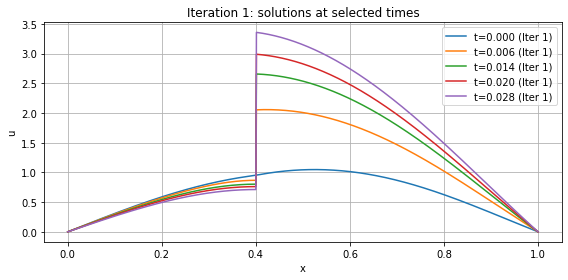
\includegraphics[width=0.48\textwidth]{assets/image-1.png} % Iter 1
    \hfill
    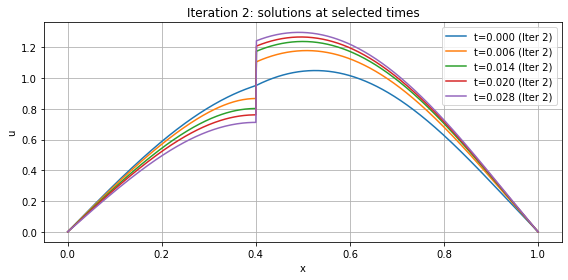
\includegraphics[width=0.48\textwidth]{assets/image-2.png} % Iter 2
    \caption{Solution profiles $u(x,t)$ at iterations 1 and 2. Each plot shows snapshots at multiple time points.}
  \end{figure}
  \textit{Initial iterations show rapid improvement.}
\end{frame}

% Slide 11: Solution Curve Evolution (Part 2)
\begin{frame}{Solution Curve Evolution (Iterations 3-5)}
  Continued from previous slide: FEM-PINN solutions vs. exact solution.
  \begin{figure}
    \centering
    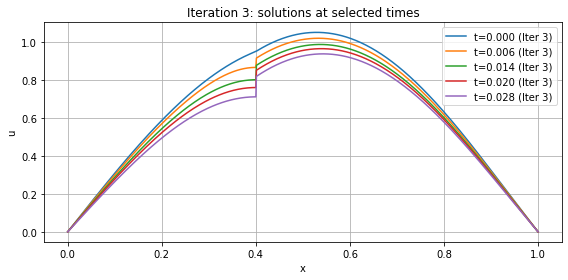
\includegraphics[width=0.48\textwidth]{assets/image-3.png} % Iter 3
    \hfill
    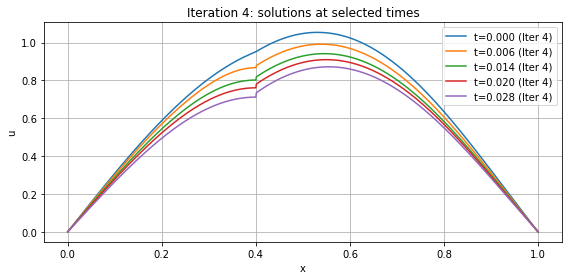
\includegraphics[width=0.48\textwidth]{assets/image-4.png} % Iter 4
    \\[1em] 
    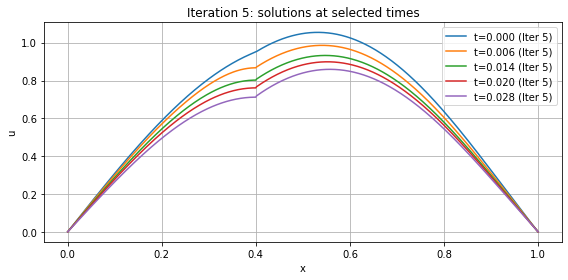
\includegraphics[width=0.48\textwidth]{assets/image-5.png} % Iter 5 (centered)
    \caption{Solution profiles $u(x,t)$ at iterations 3, 4, and 5. Each plot shows snapshots at multiple time points.}
  \end{figure}
  \textit{Later iterations show convergence towards the exact solution and smooth interface.}
\end{frame}

% Slide 12: Global Error Norms (was Slide 11)
\begin{frame}{Global Error Norms vs. Iteration}
  Errors computed for the $[0,1]$ at $t=[0,0.006,0.014,0.02,0.028]s$.
  \begin{figure}
    \centering
    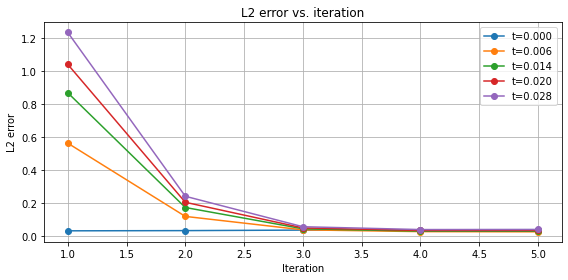
\includegraphics[width=0.48\textwidth]{assets/image-6.png}
    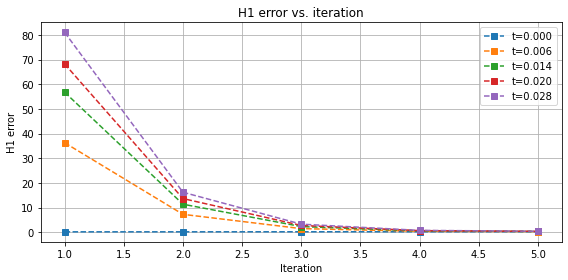
\includegraphics[width=0.48\textwidth]{assets/image-7.png}
    \caption{Left: Global $L^2$ error. Right: Global $H^1$ error.}
  \end{figure}
  \textit{Both norms show approximate exponential decay, demonstrating effective convergence.}
\end{frame}

% Slide 13: Convergence Theory & Error Propagation (was Slide 12)
\section{Convergence \& Error}
\begin{frame}{Convergence Theory \& Error Analysis}
  \begin{itemize}
    \item \textbf{Schwarz Operator (\(\mathcal{T} = \mathcal{D} \circ \mathcal{N}\)):} Defines one iteration. Converges if \(\rho(\mathcal{T})<1\).
      \[ q_{I,\text{PINN}}^{(k+1)} = \mathcal{T}[q_I^{(k)}] \]
    \item \textbf{Relaxation:} Improves stability/convergence.
      \[ q_I^{(k+1)} = \omega\,q_{I,\text{PINN}}^{(k+1)} + (1-\omega)\,q_I^{(k)} \] 
    \item \textbf{Asymptotic Error Bound:} Converged error limited by FEM/PINN inaccuracies.
      \[ \|\eta^\infty\| \lesssim \frac{\omega (L\,\delta_{\text{FEM}} + \delta_{\text{PINN}})}{1 - (\omega L + 1-\omega)} \]
      Accuracy ultimately limited by \(\max(\delta_{\text{FEM}}, \delta_{\text{PINN}})\).
  \end{itemize}
\end{frame}

% Slide 14: Conclusions & Outlook (was Slide 13) -- CORRECTED '&' to '\&'
\section{Conclusions}
\begin{frame}{Conclusions \& Future Work}
  \begin{columns}[T]
  \begin{column}{0.52\textwidth} 
    \textbf{Key Achievements:}
    \begin{itemize}
        % CORRECTED '&' to '\&' in the line below
        \item \textbf{Feasible Coupling:} FEM (Feel++) \& PINN (SciMBA) for 1D heat.
        \item \textbf{Rapid Convergence:}
            \begin{itemize}
                \item Interface error \(\mathcal{O}(10^{-2})\) in ~3 iter.
                \item Global errors near limits in 4-5 iter.
            \end{itemize}
        \item \textbf{High-Quality Solution:}
            \begin{itemize}
                \item Smooth interface.
                \item $L^2/H^1$ errors decay exponentially.
            \end{itemize}
        \item \textbf{Error Mechanism:} Understood via model; limits identified.
    \end{itemize}
  \end{column}
  \begin{column}{0.48\textwidth}
    \textbf{Future Directions:}
    \begin{itemize}
        \item \textbf{Accuracy Upgrades:}
            \begin{itemize}
                \item Refine FEM mesh/order.
                \item Enhance PINN models.
            \end{itemize}
        \item \textbf{Algorithm Speed-ups:}
            \begin{itemize}
                \item Adaptive relaxation \(\omega_k\).
                \item Advanced Schwarz (Robin, Overlapping).
            \end{itemize}
        \item \textbf{Broader Applications:}
            \begin{itemize}
                \item 2D/3D problems.
                \item Convection-diffusion.
                \item Multi-physics.
            \end{itemize}
        \item \textbf{PINN Training:}
            \begin{itemize}
                \item Adaptive sampling.
                \item Parallel/distributed methods.
            \end{itemize}
    \end{itemize}
  \end{column}
  \end{columns}
\end{frame}

% Slide 15: Acknowledgments & Questions (was Slide 14)
\begin{frame}{Acknowledgments \& Questions}
  \begin{center}
    This work leverages the capabilities of the Feel++ and SciMBA libraries. \\
    The project source code can be found at: \\ \url{https://github.com/feelpp/feelpp-scimba/tree/31-project-3}
    \vspace{2em}
    \huge Thank you! \\
    \vspace{1em}
    Questions?
  \end{center}
\end{frame}

\end{document}